%\documentclass[hyperref={pdfpagelabels=false},slidetop,9pt]{beamer}
\documentclass[slidetop,8pt]{beamer}
\usepackage[T1]{fontenc}
\usepackage[utf8]{inputenc}
\newcommand{\nom}{Porte conteneur}
\newcommand{\sequence}{03}
\newcommand{\num}{04}
\newcommand{\type}{TD}
\newcommand{\descrip}{Résolution d'un problème en utilisant des méthodes algorithmiques}
\newcommand{\competences}{Alt-C3: Concevoir un algorithme répondant à un problème précisément posé}
\usepackage{etex}
\usepackage{tikz}
\usepackage[european]{circuitikz}
\usepackage{pgf}
\usepackage[all]{xy}
\usepackage{pgfpages}
\usepackage{graphbox}
\usepackage{pdfpages}
\usepackage[adobe-utopia]{mathdesign}
\usepackage{ifthen}
\usepackage{cancel}
\usepackage{framed}
\usepackage{subfig}
\usepackage{tabularx}
\usepackage{setspace}
\usepackage{soul}
\usepackage{schemabloc}
\usepackage{eqnarray}
\usepackage[dot, phantomtext]{dashundergaps}
\usepackage{media9}
\usepackage{multimedia}

\author{Renaud Costadoat}
\institute{Lycée Dorian}

\usepackage{multido}
\usepackage{multirow}
\usepackage{multicol} % Portions de texte en colonnes
\usepackage{flafter}%floatants après la référence

\usepackage{color}
\usepackage{xcolor}
\usepackage{colortbl}

\usepackage[gen]{eurosym}
\usepackage{tikz}
%\usepackage{pstricks,pst-node,pst-tree,pst-solides3d}
\usepackage{lmodern}
\usepackage[francais]{babel}
\usepackage{pslatex}
\usetheme{renaud}
\usepackage{times}
\usepackage{amsmath}
\usepackage{verbatim}
\usepackage{moreverb}
%\usetikzlibrary{arrows,shapes}
\usepackage{graphicx}
\usepackage{psfrag}
\usepackage{wrapfig}
\usepackage{etoolbox}

\definecolor{gris25}{gray}{0.75}
\definecolor{bleu}{RGB}{18,33,98}
\definecolor{bleuf}{RGB}{42,94,171}
\definecolor{bleuc}{RGB}{231,239,247}
\definecolor{rougef}{RGB}{185,18,27}
\definecolor{rougec}{RGB}{255,188,204}%255,230,231
\definecolor{vertf}{RGB}{103,126,82}
\definecolor{vertc}{RGB}{220,255,191}

\setlength\parindent{24pt}
\parskip 7.2pt
\parindent 8pt

\newenvironment{rem}[1][\hsize]%
{%
    \def\FrameCommand
   {%
\rotatebox{90}{\textit{\textsf{Remarque}}} 
       {\color{bleuf}\vrule width 3pt}%
       \hspace{0pt}%must no space.
       \fboxsep=\FrameSep\colorbox{bleuc}%
  }%
    \MakeFramed{\hsize#1\advance\hsize-\width\FrameRestore}%
}%
{\endMakeFramed}%


\newenvironment{savoir}[1][\hsize]%
{%
    \def\FrameCommand
    {%
\rotatebox{90}{\textit{\textsf{Savoir}}} 
        {\color{bleuf}\vrule width 3pt}%
        \hspace{0pt}%must no space.
        \fboxsep=\FrameSep\colorbox{bleuc}%
    }%
    \MakeFramed{\hsize#1\advance\hsize-\width\FrameRestore}%
}%
{\endMakeFramed}%

\newenvironment{prob}[1][\hsize]%
{%
    \def\FrameCommand%
    {%
\rotatebox{90}{\textit{\textsf{Problématique}}} 
        {\color{rougef}\vrule width 3pt}%
        \hspace{0pt}%must no space.
        \fboxsep=\FrameSep\colorbox{rougec}%
    }%
    \MakeFramed{\hsize#1\advance\hsize-\width\FrameRestore}%
}%
{\endMakeFramed}%

\newenvironment{obj}[1][\hsize]%
{%
    \def\FrameCommand%
    {%
\rotatebox{90}{\textit{\textsf{Objectif}}} 
        {\color{vertf}\vrule width 3pt}%
        \hspace{0pt}%must no space.
        \fboxsep=\FrameSep\colorbox{vertc}%
    }%
    \MakeFramed{\hsize#1\advance\hsize-\width\FrameRestore}%
}%
{\endMakeFramed}%

\newenvironment{defi}[1][\hsize]%
{%
    \def\FrameCommand%
    {%
\rotatebox{90}{\textit{\textsf{Definition}}} 
        {\color{bleuf}\vrule width 3pt}%
        \hspace{0pt}%must no space.
        \fboxsep=\FrameSep\colorbox{rougec}%
    }%
    \MakeFramed{\hsize#1\advance\hsize-\width\FrameRestore}%
}%
{\endMakeFramed}%


\newenvironment{hypo}[1][\hsize]%
{%
    \def\FrameCommand%
    {%
\rotatebox{90}{\textit{\textsf{Hypothèse\\}}} 
        {\color{bleuf}\vrule width 3pt}%
        \hspace{0pt}%must no space.
        \fboxsep=\FrameSep\colorbox{bleuc}%
    }%
    \MakeFramed{\hsize#1\advance\hsize-\width\FrameRestore}%
}%
{\endMakeFramed}%


\newenvironment{prop}[1][\hsize]%
{%
    \def\FrameCommand%
    {%
\rotatebox{90}{\textit{\textsf{Propriété}}} 
        {\color{bleuf}\vrule width 3pt}%
        \hspace{0pt}%must no space.
        \fboxsep=\FrameSep\colorbox{bleuc}%
    }%
    \MakeFramed{\hsize#1\advance\hsize-\width\FrameRestore}%
}%
{\endMakeFramed}%

\newenvironment{props}[1][\hsize]%
{%
    \def\FrameCommand%
    {%
\rotatebox{90}{\textit{\textsf{Propriétés}}} 
        {\color{bleuf}\vrule width 3pt}%
        \hspace{0pt}%must no space.
        \fboxsep=\FrameSep\colorbox{bleuc}%
    }%
    \MakeFramed{\hsize#1\advance\hsize-\width\FrameRestore}%
}%
{\endMakeFramed}%

\newenvironment{exemple}[1][\hsize]%
{%
    \def\FrameCommand%
    {%
\rotatebox{90}{\textit{\textsf{Exemple}}} 
        {\color{vertf}\vrule width 3pt}%
        \hspace{0pt}%must no space.
        \fboxsep=\FrameSep\colorbox{vertc}%
    }%
    \MakeFramed{\hsize#1\advance\hsize-\width\FrameRestore}%
}%
{\endMakeFramed}%

\newenvironment{resultat}[1][\hsize]%
{%
    \def\FrameCommand%
    {%
\rotatebox{90}{\textit{\textsf{Resultat}}} 
        {\color{rougef}\vrule width 3pt}%
%        {\color{bleuf}\vrule width 3pt}%
        \hspace{0pt}%must no space.
        \fboxsep=\FrameSep\colorbox{rougec}%
    }%
    \MakeFramed{\hsize#1\advance\hsize-\width\FrameRestore}%
}%
{\endMakeFramed}%

\newenvironment{methode}[1][\hsize]%
{%
    \def\FrameCommand%
    {%
\rotatebox{90}{\textit{\textsf{Méthode\\}}} 
        {\color{rougef}\vrule width 3pt}%
        \hspace{0pt}%must no space.
        \fboxsep=\FrameSep\colorbox{rougec}%
    }%
    \MakeFramed{\hsize#1\advance\hsize-\width\FrameRestore}%
}%
{\endMakeFramed}%

\newenvironment{theo}[1][\hsize]%
{%
    \def\FrameCommand%
    {%
\rotatebox{90}{\textit{\textsf{Théorème\\}}} 
        {\color{rougef}\vrule width 3pt}%
        \hspace{0pt}%must no space.
        \fboxsep=\FrameSep\colorbox{rougec}%
    }%
    \MakeFramed{\hsize#1\advance\hsize-\width\FrameRestore}%
}%
{\endMakeFramed}%

\newenvironment{warn}[1][\hsize]%
{%
    \def\FrameCommand%
    {%
\rotatebox{90}{\textit{\textsf{Attention\\}}} 
        {\color{rougef}\vrule width 3pt}%
        \hspace{0pt}%must no space.
        \fboxsep=\FrameSep\colorbox{rougec}%
    }%
    \MakeFramed{\hsize#1\advance\hsize-\width\FrameRestore}%
}%
{\endMakeFramed}%

% \usepackage{pstricks}
%\usepackage{minitoc}
% \setcounter{minitocdepth}{4}

\setcounter{tocdepth}{2}

% \mtcselectlanguage{french} 

%\usepackage{draftcopy}% "Brouillon"
% \usepackage{floatflt}
\usepackage{psfrag}
%\usepackage{listings} % Permet d'insérer du code de programmation
\renewcommand{\baselinestretch}{1.2}

% Changer la numérotation des figures :
% ------------------------------------
% \makeatletter
% \renewcommand{\thefigure}{\ifnum \c@section>\z@ \thesection.\fi
%  \@arabic\c@figure}
% \@addtoreset{figure}{section}
% \makeatother
 


%%%%%%%%%%%%
% Définition des vecteurs %
%%%%%%%%%%%%
 \newcommand{\vect}[1]{\overrightarrow{#1}}

%%%%%%%%%%%%
% Définition des torseusr %
%%%%%%%%%%%%

 \newcommand{\torseur}[1]{%
\left\{{#1}\right\}
}

\newcommand{\torseurcin}[3]{%
\left\{\mathcal{#1} \left(#2/#3 \right) \right\}
}

\newcommand{\torseurstat}[3]{%
\left\{\mathcal{#1} \left(#2\rightarrow #3 \right) \right\}
}

 \newcommand{\torseurc}[8]{%
%\left\{#1 \right\}=
\left\{
{#1}
\right\}
 = 
\left\{%
\begin{array}{cc}%
{#2} & {#5}\\%
{#3} & {#6}\\%
{#4} & {#7}\\%
\end{array}%
\right\}_{#8}%
}

 \newcommand{\torseurcol}[7]{
\left\{%
\begin{array}{cc}%
{#1} & {#4}\\%
{#2} & {#5}\\%
{#3} & {#6}\\%
\end{array}%
\right\}_{#7}%
}

 \newcommand{\torseurl}[3]{%
%\left\{\mathcal{#1}\right\}_{#2}=%
\left\{%
\begin{array}{l}%
{#1} \\%
{#2} %
\end{array}%
\right\}_{#3}%
}

 \newcommand{\vectv}[3]{%
\vect{V\left( {#1} \in {#2}/{#3}\right)}
}


\newcommand{\vectf}[2]{%
\vect{R\left( {#1} \rightarrow {#2}\right)}
}

\newcommand{\vectm}[3]{%
\vect{\mathcal{M}\left( {#1}, {#2} \rightarrow {#3}\right)}
}


 \newcommand{\vectg}[3]{%
\vect{\Gamma \left( {#1} \in {#2}/{#3}\right)}
}

 \newcommand{\vecto}[2]{%
\vect{\Omega\left( {#1}/{#2}\right)}
}

\newcommand{\reponse}[1][4]
{
\multido{}{#1}
{
\begin{center}
\makebox[0.9\linewidth]{\dotfill} \end{center}
}}


% }$$\left\{\mathcal{#1} \right\}_{#2} =%
% \left\{%
% \begin{array}{c}%
%  #3 \\%
%  #4 %
% \end{array}%
% \right\}_{#5}}


%  ------------------------------------------
% | Modification du formatage des sections : | 
%  ------------------------------------------

% Grands titres :
% ---------------

\newcommand{\titre}[1]{%
\begin{center}
      \bigskip
      \rule{\textwidth}{1pt}
      \par\vspace{0.1cm}
      
      \textbf{\large #1}
      \par\rule{\textwidth}{1pt}
    \end{center}
    \bigskip
  }

% Supprime le numéro du chapitre dans la numérotation des sections:
% -----------------------------------------------------------------
\makeatletter
\renewcommand{\thesection}{\@arabic\c@section}
\makeatother


% \titleformat{\chapter}[display]
% {\normalfont\Large\filcenter}
% {}
% {1pc}
% {\titlerule[1pt]
%   \vspace{1pc}%
%   \Huge}[\vspace{1ex}%
% \titlerule]


%%%% Chapitres Comme PY Pechard %%%%%%%%%
% numéro du chapitre
\DeclareFixedFont{\chapnumfont}{OT1}{phv}{b}{n}{80pt}
% pour le mot « Chapitre »
\DeclareFixedFont{\chapchapfont}{OT1}{phv}{m}{it}{40pt}
% pour le titre
\DeclareFixedFont{\chaptitfont}{T1}{phv}{b}{n}{25pt}

\definecolor{gris}{gray}{0.75}
\setbeamertemplate{section in toc}[sections numbered]

\newlength{\RoundedBoxWidth}
\newsavebox{\GrayRoundedBox}
\newenvironment{GrayBox}[1][\dimexpr\textwidth-4.5ex]%
   {\setlength{\RoundedBoxWidth}{\dimexpr#1}
    \begin{lrbox}{\GrayRoundedBox}
       \begin{minipage}{\RoundedBoxWidth}}%
   {   \end{minipage}
    \end{lrbox}
    \begin{center}
    \begin{tikzpicture}%
       \draw node[draw=bleuf,fill=bleuc,rounded corners,%
             inner sep=2ex,text width=\RoundedBoxWidth]%
             {\usebox{\GrayRoundedBox}};
    \end{tikzpicture}
    \end{center}}
    
\ifdef{\prive}{\pgfpagesuselayout{2 on 1}[a4paper,border shrink=0mm]}
\ifdef{\prive}{\setbeamertemplate{navigation symbols}{}}
\setbeamertemplate{itemize item}[ball]
%\setbeamertemplate{blocks}[rounded]%[shadow=true]
\setbeamercolor{block title}{fg=white,bg=grisf}        % titre block normal 
\setbeamercolor{block body}{fg=grisf,bg=grisc!50}      % corps block normal
\setbeamercolor{block body alerted}{fg=white,bg=warning}   % idem pour un block alerte

\title{\nom}
\date{S\sequence \ - \type\num}

\begin{document}
\shorthandoff{:!}
\bibliographystyle{abbrvnat-fr}

\usebackgroundtemplate%
{%
    \centering
\includegraphics[width=\paperwidth]{../../img/fond2}%
}

{
\setbeamertemplate{navigation symbols}{}
\setbeamertemplate{headline}[pagetitre]
\setbeamertemplate{footline}[pagetitre]
\usebackgroundtemplate{\centering
\includegraphics[width=\paperwidth]{../../img/fond}}
\frame{\titlepage}
}



\section{Méthode des rectangles} 

\begin{frame}[fragile]
\frametitle{Méthode des rectangles}

Dans cette méthode, on calcule l'intégrale numérique en réalisant une somme de surfaces de rectangles. Le domaine d'intégration est découpé en intervalles et on fait comme si la fonction restait constante sur chaque intervalle.

Sur chaque intervalle, on réalise ainsi l'approximation suivante :

$\int_{a}^{b} f(x).dx \approx (b-a).f(\alpha)$, où $\alpha$ est une abscisse appartenant à l'intervalle limité par $a$ et $b$.

Nous nous limiterons ici aux cas où $\alpha=a$, $\alpha=b$ ou $\alpha=\dfrac{a+b}{2}$.

\begin{minipage}{0.6\linewidth}
Comme exemple, nous allons réaliser un programme d'intégration pour $\alpha=a$ et nous visualiserons les rectangles.

Pour tracer un rectangle ABCD (voir figure ci-dessous), il suffit de faire un plot avec les coordonnées de A, B, C, D et A. On termine par A pour fermer le tracé.
\end{minipage}\hfill
\begin{minipage}{0.35\linewidth}
\begin{center}
	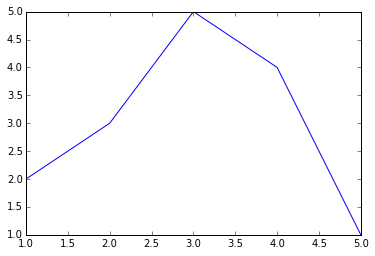
\includegraphics[width=0.9\linewidth]{img/courbe0}
\end{center}
\end{minipage}
\end{frame}

\begin{frame}[fragile]
\frametitle{Méthode des rectangles}

\begin{minipage}{0.3\linewidth}
Cas $\alpha=a$ \\
\begin{center}
	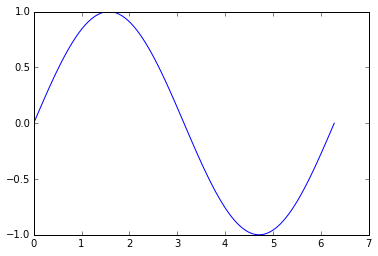
\includegraphics[width=0.9\linewidth]{img/courbe1}
\end{center}
\end{minipage}\hfill
\begin{minipage}{0.3\linewidth}
Cas $\alpha=b$ \\
\begin{center}
	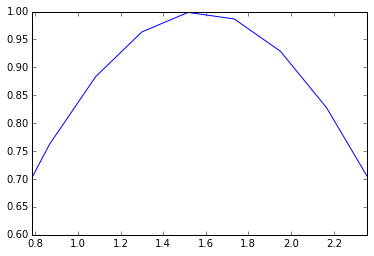
\includegraphics[width=0.9\linewidth]{img/courbe2}
\end{center}
\end{minipage}\hfill
\begin{minipage}{0.3\linewidth}
Cas $\alpha=\dfrac{a+b}{2}$ \\
\begin{center}
	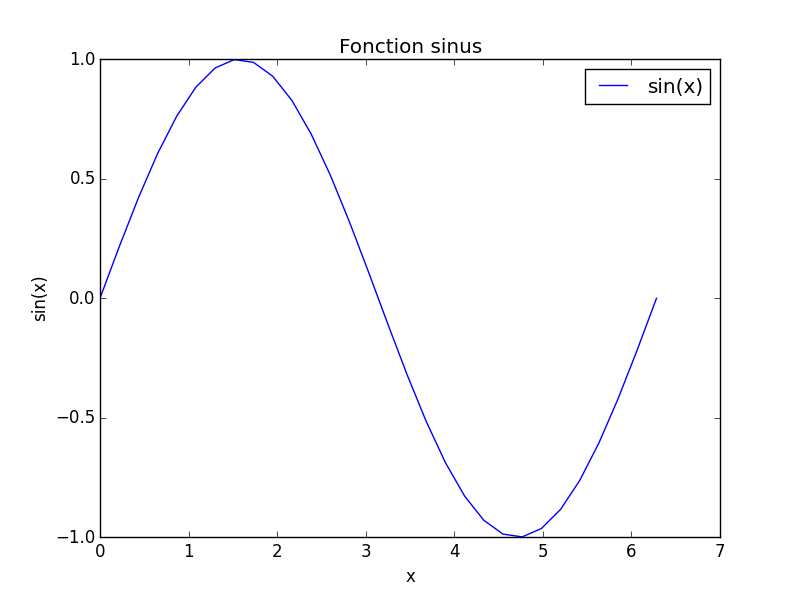
\includegraphics[width=0.9\linewidth]{img/courbe3}
\end{center}
\end{minipage}

La méthode $\alpha=\dfrac{a+b}{2}$ est plus difficile à mettre en \oe uvre car, il faut alors découper en deux les intervalles d'intégration. Souvent $a$ et $b$ sont des entiers consécutifs et cela empêche cette division.

L'objectif de la méthode des rectangles est de faire la somme de la surface de ces carrés au fur et à mesure de l'avancement du programme.
\end{frame}

\begin{frame}[fragile]
\frametitle{Méthode des rectangles ($\alpha=a$)}

Création de la fonction \verb?y? et de la variable \verb?x?.
\begin{GrayBox}[0.85\textwidth]
\begin{verbatimtab}[3]
xmin, xmax, nbx = 0, 3*pi/2, 2006
x = linspace(xmin, xmax, nbx)
y = cos(x)
plot(x,y,"bo-")
\end{verbatimtab}
\end{GrayBox}

Calcul de l'intégrale \verb?int?.
\begin{GrayBox}[0.85\textwidth]
\begin{verbatimtab}[3]
nbi = nbx - 1 # nombre d'intervalles
int = linspace(1, 1, nbx)
int[0]=0

for i in range(nbi):
    int[i+1] = int[i] + y[i]*(x[i+1]-x[i])
\end{verbatimtab}
\end{GrayBox}

\end{frame}

\begin{frame}[fragile]
\frametitle{Méthode des rectangles ($\alpha=b$)}

Modifier le programme pour prendre $\alpha=b$.
\begin{GrayBox}[0.85\textwidth]
\begin{verbatimtab}[3]
xmin, xmax, nbx = 0, 3*pi/2, 2006
x = linspace(xmin, xmax, nbx)
y = cos(x)
plot(x,y,"bo-")

nbi = nbx - 1 # nombre d'intervalles
int = linspace(1, 1, nbx)
int[0]=0

for i in range(nbi):
    int[i+1] = int[i] + y[i+1]*(x[i+1]-x[i])
\end{verbatimtab}
\end{GrayBox}

\end{frame}

\begin{frame}[fragile]
\frametitle{Méthode des trapèzes}

Coder la méthode des trapèzes.
\vspace{7cm}

\end{frame}

\section{Création de courbes} 

\begin{frame}[fragile]
\frametitle{Création de courbes}

L'instruction \verb? plot()? permet de tracer des courbes qui relient des points dont les abscisses et ordonnées sont fournies dans des tableaux.

\begin{minipage}{0.5\linewidth}
\begin{GrayBox}[0.85\textwidth]
\begin{verbatimtab}[3]
import numpy as np
import matplotlib.pyplot as plt

x = np.array(range(1,6))
y = np.array([2, 3, 5, 4, 1])
plt.plot(x, y)

plt.show() # affiche la figure
\end{verbatimtab}
\end{GrayBox}
\end{minipage}\hfill
\begin{minipage}{0.46\linewidth}
\begin{center}
 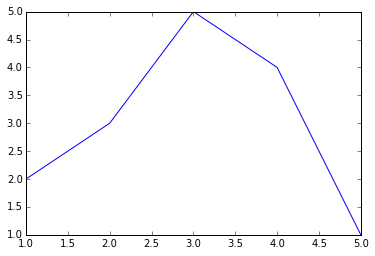
\includegraphics[width=0.9\linewidth]{img/courbe0}
\end{center}
\end{minipage}

\end{frame}

\begin{frame}[fragile]
\frametitle{Création de courbes}

De la même manière, il est possible de tracer une fonction \verb? sin(x)?.

\begin{minipage}{0.5\linewidth}
\begin{GrayBox}[0.85\textwidth]
\begin{verbatimtab}[3]
import numpy as np
import matplotlib.pyplot as plt

x = np.linspace(0, 2*np.pi, 100)
y = np.sin(x)
plt.plot(x, y)

plt.show()
\end{verbatimtab}
\end{GrayBox}
\end{minipage}\hfill
\begin{minipage}{0.46\linewidth}
\begin{center}
 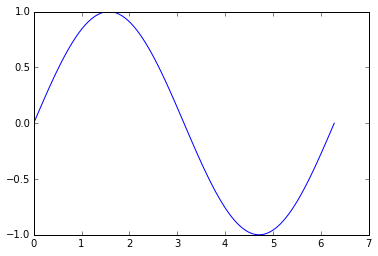
\includegraphics[width=0.9\linewidth]{img/courbe1}
\end{center}
\end{minipage}

\end{frame}

\begin{frame}[fragile]
\frametitle{Définition du domaine des axes}

Les fonction \verb? xlim(xmin, xmax)? et \verb? ylim(ymin, ymax)? permettent de fixer indépendamment les domaines des abscisses et des ordonnées.

\begin{minipage}{0.5\linewidth}
\begin{GrayBox}[0.85\textwidth]
\begin{verbatimtab}[3]
import numpy as np
import matplotlib.pyplot as plt

x = np.linspace(0, 2*np.pi, 30)
y = np.sin(x)
plt.plot(x, y)
plt.xlim(np.pi/4, 3*np.pi/4)
plt.ylim(0.6, 1)

plt.show()
\end{verbatimtab}
\end{GrayBox}
\end{minipage}\hfill
\begin{minipage}{0.46\linewidth}
\begin{center}
 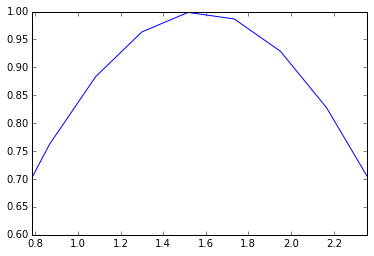
\includegraphics[width=0.9\linewidth]{img/courbe2}
\end{center}
\end{minipage}

\end{frame}

\begin{frame}[fragile]
\frametitle{Ajouter un titre, une légende ou des labels}

Les courbes tracées doivent être accompagnée d'informations afin de pouvoir être interprétées.

\begin{minipage}{0.5\linewidth}
\begin{GrayBox}[0.85\textwidth]
\begin{verbatimtab}[3]
import numpy as np
import matplotlib.pyplot as plt

x = np.linspace(0, 2*np.pi, 30)
y = np.sin(x)
plt.plot(x, y, label="sin(x)")
plt.legend()
plt.title("Fonction sinus")
plt.xlabel("x")
plt.ylabel("sin(x)")

plt.show()
\end{verbatimtab}
\end{GrayBox}
\end{minipage}\hfill
\begin{minipage}{0.46\linewidth}
\begin{center}
 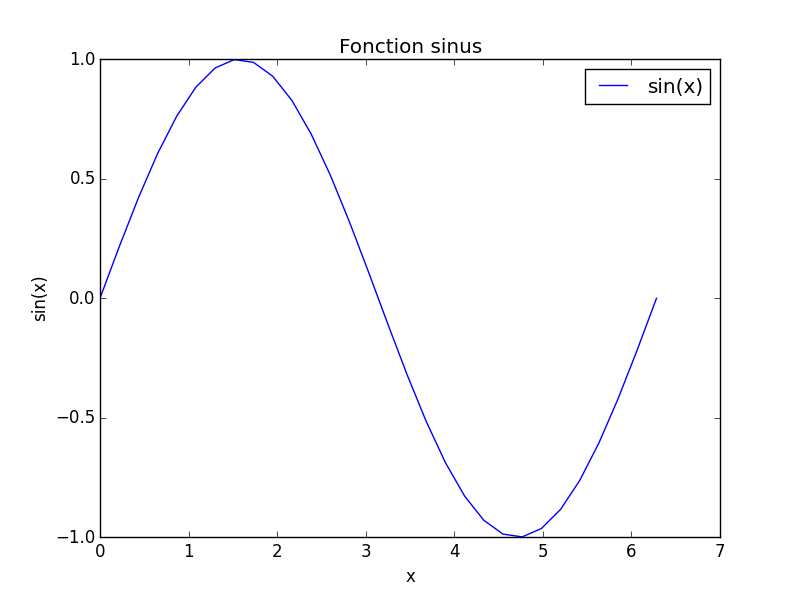
\includegraphics[width=0.9\linewidth]{img/courbe3}
\end{center}
\end{minipage}

\end{frame}

\begin{frame}[fragile]
\frametitle{Style des lignes}

Il est nécessaire de modifier le style des lignes afin de les identifier.

\begin{minipage}{0.6\linewidth}
\begin{GrayBox}[0.85\textwidth]
\begin{verbatimtab}[3]
import numpy as np
import matplotlib.pyplot as plt

x = np.linspace(0, 2*np.pi, 20)
y = np.cos(x)
plt.plot(x, y, "o-", label="-")
plt.plot(x, y-0.5, "o--", label="--")
plt.plot(x, y-1, "o:", label=":")
plt.plot(x, y-1.5, "o-.", label="-.")
plt.plot(x, y-2, "o", label="no line")
plt.legend()

plt.show()
\end{verbatimtab}
\end{GrayBox}
\end{minipage}\hfill
\begin{minipage}{0.36\linewidth}
\begin{center}
 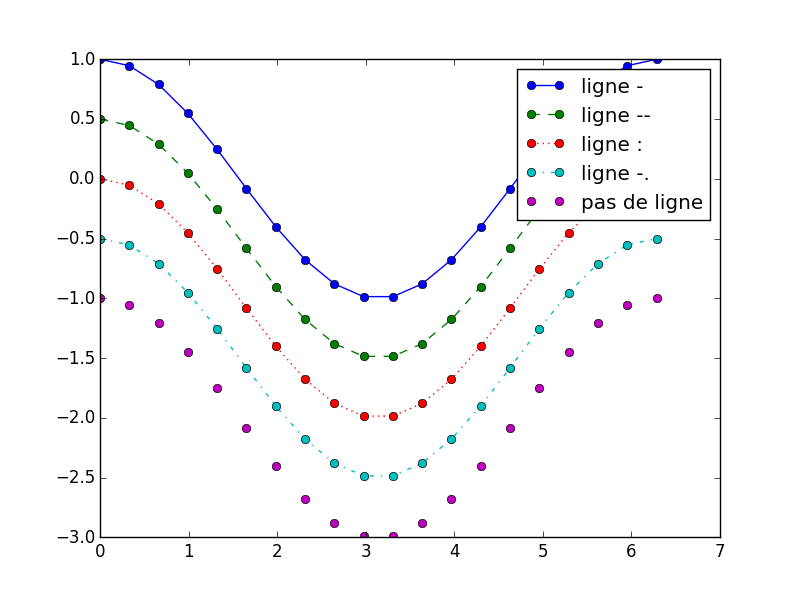
\includegraphics[width=1\linewidth]{img/courbe4}
\end{center}
\end{minipage}

\end{frame}

\begin{frame}[fragile]
\frametitle{Tracé de formes}

Comme la fonction \verb? plot()? ne fait que relier des points, il est possible de lui fournir plusieurs points avec la même abscisse.

\begin{minipage}{0.6\linewidth}
\begin{GrayBox}[0.85\textwidth]
\begin{verbatimtab}[3]
x = np.array([0, 1, 1, 0, 0])
y = np.array([0, 0, 1, 1, 0])
plt.plot(x, y)

theta = np.linspace(0, 2*np.pi, 40)
x = np.cos(theta)
y = np.sin(theta)
plt.plot(x, y)
plt.axis("equal")
plt.show()
\end{verbatimtab}
\end{GrayBox}
\end{minipage}\hfill
\begin{minipage}{0.36\linewidth}
\begin{center}
 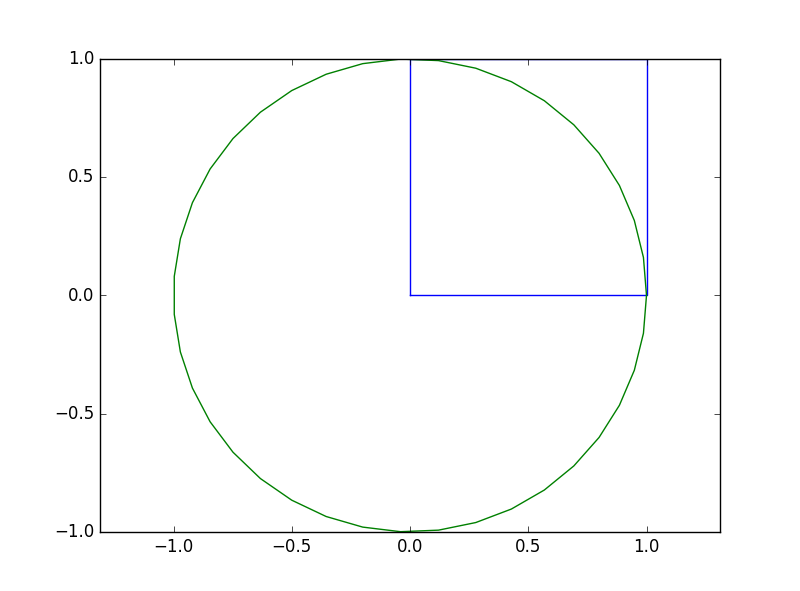
\includegraphics[width=1\linewidth]{img/courbe5}
\end{center}
\end{minipage}

\end{frame}

\begin{frame}[fragile]
\frametitle{Tracé de formes}

Déterminer les $k_i$, $\omega_i$, $\varphi_i$ et $c_i$ et coder le tracé du profil de vitesse $v(t)=\dot{x}(t)$ suivant:
\begin{itemize}
 \item $0\leq t \leq 1: \dot{x}(t)=k_1.sin(\omega_1.t+\varphi_1)+c_1$,
 \item $1 < t \leq 3: \dot{x}(t)=v_{max}$,
 \item $3 < t \leq 5: \dot{x}(t)=k_2.sin(\omega_2.t+\varphi_2)+c_2$.
\end{itemize}


\begin{minipage}{0.6\linewidth}
\begin{GrayBox}[0.85\textwidth]

\vspace{3cm}

\end{GrayBox}
\end{minipage}\hfill
\begin{minipage}{0.36\linewidth}
\begin{center}
 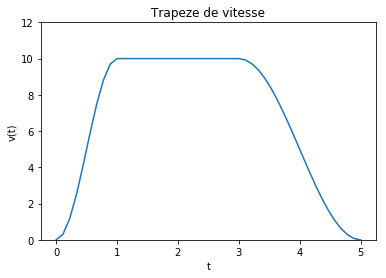
\includegraphics[width=1\linewidth]{img/courbe6}
\end{center}
\end{minipage}

\end{frame}

\end{document}
